\documentclass{article}
\usepackage{color,soul}
\usepackage{amsmath}
\usepackage{amsfonts} 
\usepackage{eqnarray}
\usepackage{bm}
\usepackage{multirow}
\usepackage{graphicx}
\usepackage{booktabs}
\usepackage{subcaption}
\usepackage{listings}
\usepackage[margin=0.5in]{geometry}

\title{School of Electrical and Computer Engineering\\
Purdue University, WL, IN, USA}
\author{Nahian Ibn Hasan\\
Email: hasan34@purdue.edu\\
PUID: 0032764564\\
ECE66100 - Computer Vission\\
Fall 2022\\
Homework-2}
\date{\today}

\begin{document}
\maketitle
\section{Objective}
In this homework, we will estimate homographies between a given set of images and use the estimated homographies to transform images.
\section{Theory}
Given a point $x$ in the planar scene and the corresponding point in the $x'$ in the image plane, the homographic transformation can be written as
\begin{equation}
	X' = HX.
	\label{eq:h_transform}
\end{equation}
Here, $x$ and $x'$ are represented in homographic coordinates and $H$ is the homographic matrix. Therefore,
\begin{eqnarray}
	X = \begin{bmatrix}
		x_1 \\ x_2 \\x_3
	\end{bmatrix};
	X' = \begin{bmatrix}
		x_1' \\ x_2' \\ x_3'
	\end{bmatrix};
	H = \begin{bmatrix}
		h_{11} & h_{12} & h_{13} \\
		h_{21} & h_{22} & h_{23} \\
		h_{31} & h_{32} & h_{33}
	\end{bmatrix}.
\end{eqnarray}
The expression in equation \ref{eq:h_transform} becomes
\begin{subequations}
\begin{eqnarray}
	x_1' = h_{11}x_1 + h_{12}x_2 + h_{13}x_3\\
	x_2' = h_{21}x_1 + h_{22}x_2 + h_{23}x_3\\
	x_3' = h_{31}x_1 + h_{32}x_2 + h_{33}x_3
	\label{eq:h_transform_2}
\end{eqnarray}
\end{subequations}
Now, we can transform these homographic coordinates to physical coordinates by the following transformations-
\begin{eqnarray}
	x = \frac{x_1}{x_3};
	y = \frac{x_2}{x_3};
	x' = \frac{x_1'}{x_3'};
	y' = \frac{x_2'}{x_3'}
	\label{eq:h_transform_3}
\end{eqnarray}
Here, $(x,y)$ is the physical scene coordinate and $(x',y')$ is the physical image plane coordinate. Hence, using equations in \ref{eq:h_transform_2} and \ref{eq:h_transform_3}, we get
\begin{subequations}
	\begin{eqnarray}
		x' = \frac{h_{11}x_1 + h_{12}x_2 + h_{13}x_3}{h_{31}x_1 + h_{32}x_2 + h_{33}x_3}\\
		y' = \frac{h_{21}x_1 + h_{22}x_2 + h_{23}x_3}{h_{31}x_1 + h_{32}x_2 + h_{33}x_3}
	\end{eqnarray}
\end{subequations}
Or,
\begin{subequations}
	\begin{eqnarray}
		x' = \frac{h_{11}x + h_{12}y + h_{13}}{h_{31}x + h_{32}y + h_{33}}\\
		y' = \frac{h_{21}x + h_{22}y + h_{23}}{h_{31}x + h_{32}y + h_{33}}
	\end{eqnarray}
\end{subequations}
Or,
\begin{subequations}
	\begin{eqnarray}
		h_{11}x + h_{12}y + h_{13} - h_{31}xx' - h_{32}yx' - h_{33}x' = 0\\
		h_{21}x + h_{22}y + h_{23} - h_{31}xy' - h_{32}yy' - h_{33}y' = 0
	\label{eq:h_transform_4}
	\end{eqnarray}
\end{subequations}
Let's assume $h_{33}=1$. Now, if we have 4 pairs of physical coordinates in the physical scene and physical image plane, we can evaluate equation \ref{eq:h_transform_4} at those four pairs and end-up with 8 equations, which can be solved later to find out the coefficients of homographic matrix $H$. Let's assume the four pairs are $\{(x_1,y_1),(x_1',y_1')\}$, $\{(x_2,y_2),(x_2',y_2')\}$, $\{(x_3,y_3),(x_3',y_3')\}$ and $\{(x_4,y_4),(x_4',y_4')\}$. Hence, the resultant equations can be expressed in matrix notation as follows-
\begin{equation}
	\begin{bmatrix}
		x_1 & y_1 & 1 & 0 & 0 & 0 & -x_1x_1' & -y_1x_1'\\
		0 & 0 & 0 & x_1 & y_1 & 1 & -x_1y_1' & -y_1y_1'\\
		x_2 & y_2 & 1 & 0 & 0 & 0 & -x_2x_2' & -y_2x_2'\\
		0 & 0 & 0 & x_2 & y_2 & 1 & -x_2y_2' & -y_2y_2'\\
		x_3 & y_3 & 1 & 0 & 0 & 0 & -x_3x_3' & -y_3x_3'\\
		0 & 0 & 0 & x_3 & y_3 & 1 & -x_3y_3' & -y_3y_3'\\
		x_4 & y_4 & 1 & 0 & 0 & 0 & -x_4x_4' & -y_4x_4'\\
		0 & 0 & 0 & x_4 & y_4 & 1 & -x_4y_4' & -y_4y_4'\\
	\end{bmatrix}
	\begin{bmatrix}
		h_{11} \\ h_{12} \\ h_{13} \\ h_{21} \\ h_{22} \\ h_{23} \\ h_{31} \\ h_{32}
	\end{bmatrix} = 
	\begin{bmatrix}
		x_1' \\ y_1' \\ x_2' \\ y_2' \\ x_3' \\ y_3' \\ x_4' \\y_4'
	\end{bmatrix}
	\label{eq:h_transform_5}
\end{equation}
Or,
\begin{equation}
	Ax = b.
\end{equation}
The system of linear equations in \ref{eq:h_transform_5} can be solved as $x = A^{-1}b$.

We find the four corresponding pairs in both scene plane and image plane and then apply equation \ref{eq:h_transform_5} to solve for the unknowns in $H$ matrix.
\section{Task 1}
The following table lists the data points used as features to construct the hographic transformations among the provided images.
\begin{table}[!htbp]
  \caption{Corresponding Points}
    \begin{tabular}{p{0.20\linewidth}p{0.20\linewidth}p{0.50\linewidth}}
        \toprule
        \textbf{Image} & \textbf{Point} & \textbf{Physical Scene Plane Coordinate $(x, y)$}\\
        \midrule
    	\multirow{4}{*}{building.jpg}& P & (240,196) \\
    	& Q & (235,371) \\ & R & (294,375) \\ & S & (299,213)\\
    	\hline
    	\multirow{4}{*}{nighthawks.jpg}& P & (76,180) \\
    	& Q & (78,652) \\ & R & (804,621) \\ & S & (802,219)\\
    	\hline
    	\multirow{4}{*}{building undistorted.jpg}& P & (0,0) \\
    	& Q & (0,176) \\ & R & (55,176) \\ & S & (55,0)\\
    	\hline
    	\multirow{4}{*}{nighthawks undistorted.jpg}& P & (0,0) \\
    	& Q & (0,474) \\ & R & (730,474) \\ & S & (730,0)\\
    	\bottomrule
    \end{tabular}
  \label{tab:conductivities}
\end{table}
\newpage
\subsection{Input Images}
\begin{figure}[!htbp]
     \centering
    \captionsetup[subfigure]{labelformat=empty}
    \subcaptionbox{\large\textbf{1a}}{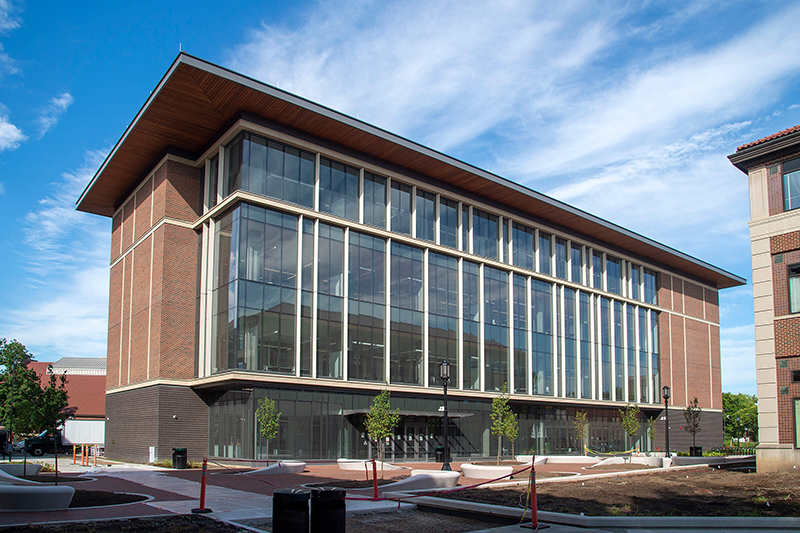
\includegraphics[width=0.45\textwidth]{../building.jpg}}
    \subcaptionbox{\large\textbf{1b}}{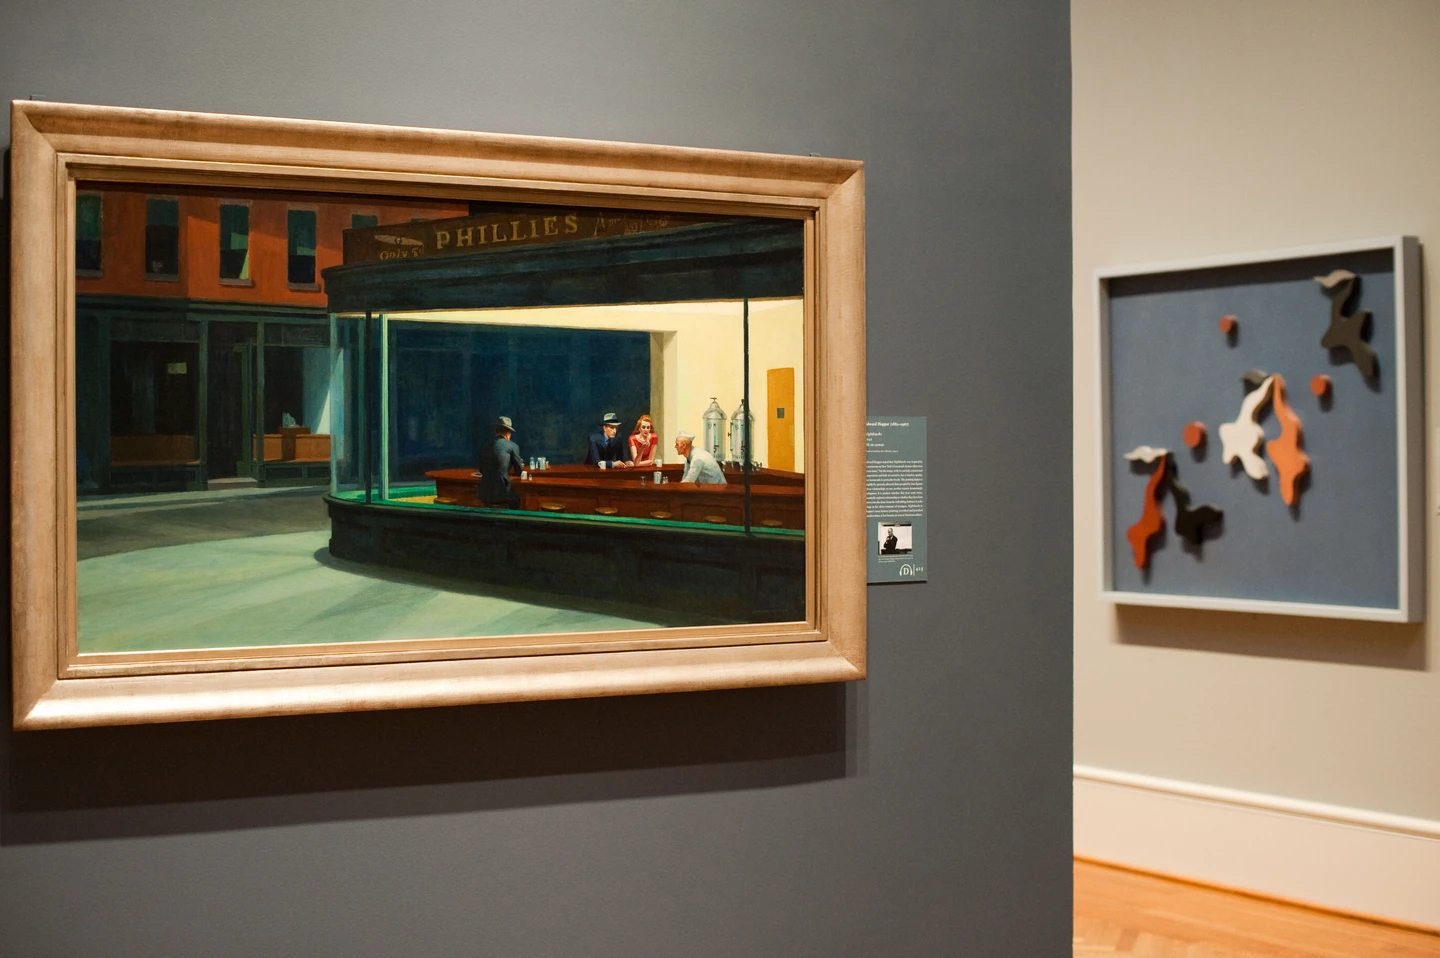
\includegraphics[width=0.45\textwidth]{../nighthawks.jpg}}
    \caption{Distorted Input Images}
\end{figure}

\subsection{Undistorted Images}
\begin{figure}[!htbp]
     \centering
    \captionsetup[subfigure]{labelformat=empty}
    \subcaptionbox{\large\textbf{a}}{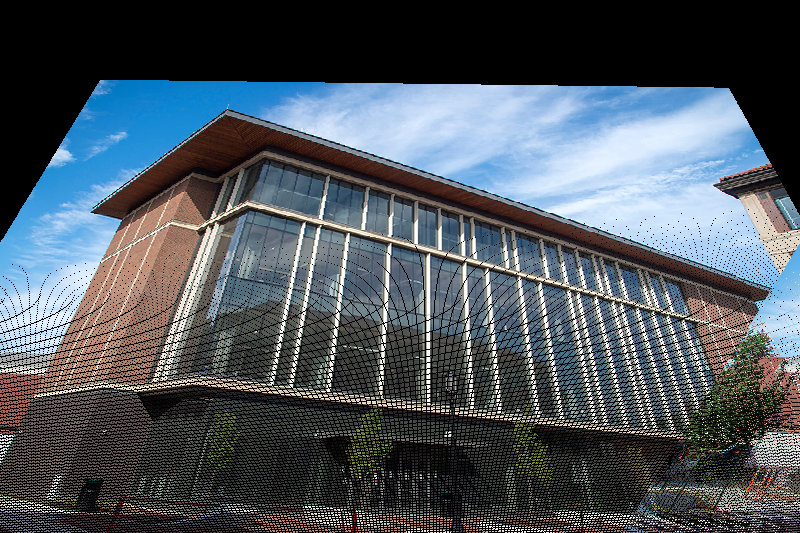
\includegraphics[width=0.45\textwidth]{../building_transformed.png}}
    \subcaptionbox{\large\textbf{b}}{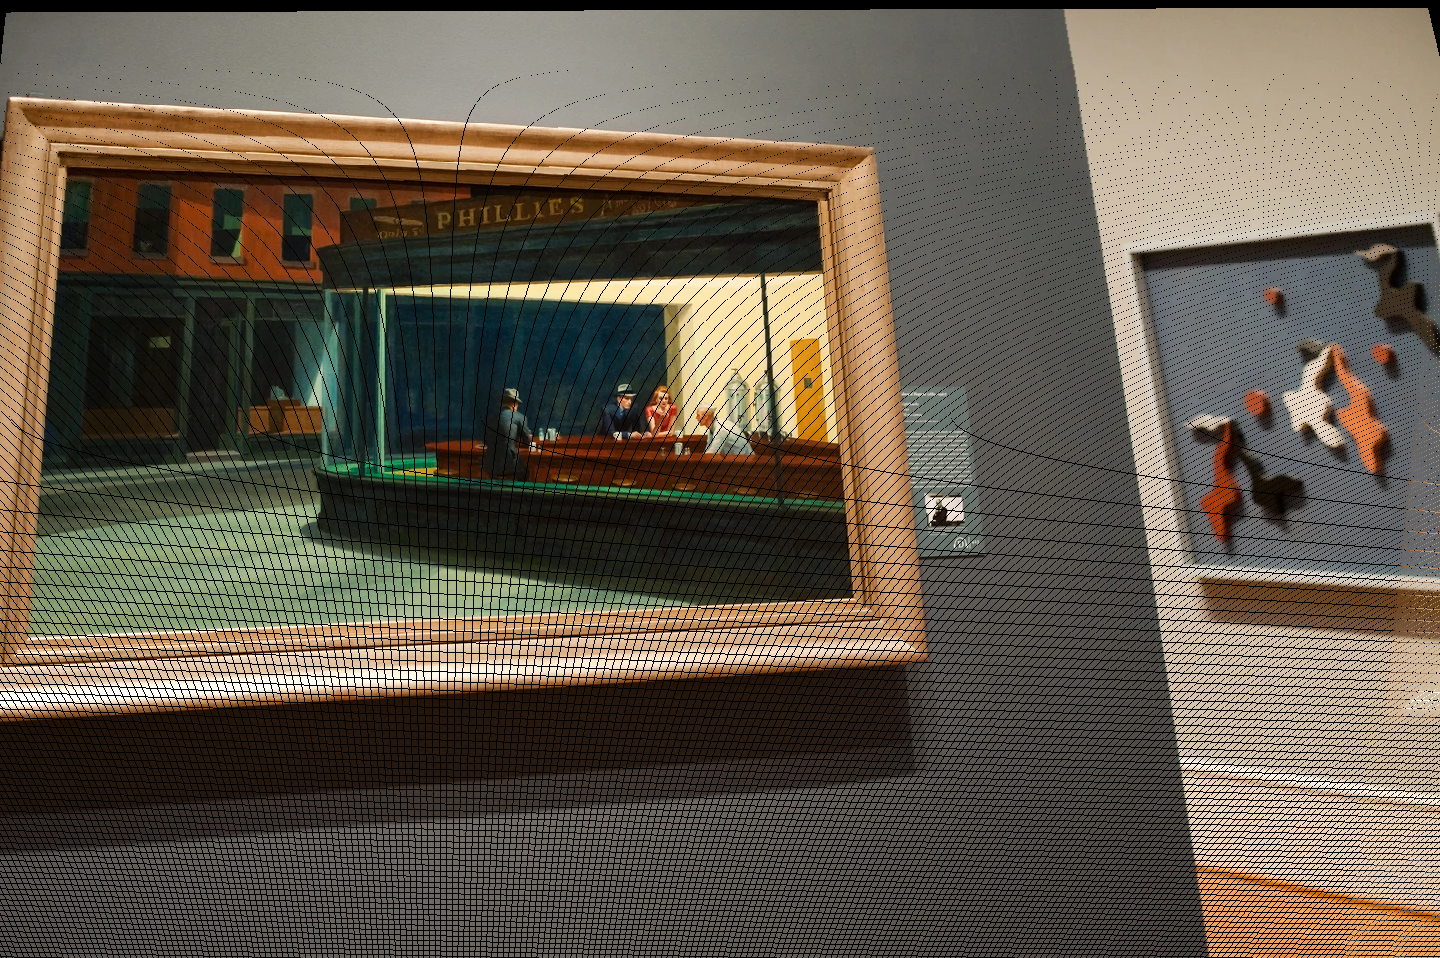
\includegraphics[width=0.45\textwidth]{../nighthawks_transformed.png}}
    \caption{Undistorted Images}
\end{figure}


\newpage
\section{Two Step Method}
The projective distortion can be eliminated by the homography that takes the vanishing line (VL) back to $l_\infty$. The homography that takes the VL to inifinity is 
\begin{equation}
	H = 
	\begin{bmatrix}
		1 & 0 & 0\\0 & 1 & 0\\l_1 & l_2 & l_3
	\end{bmatrix},
\end{equation}
where l=$\begin{bmatrix}
l_1 \\ l_2 \\l_3
\end{bmatrix}$ is the VL. However, lines are transformed by $H^{-T}$.Therefore,
\begin{equation}
	H^{-1} = \begin{bmatrix}
		1 & 0 & 0\\0 & 1 & 0\\-l_1/l_3 & -l_2/l_3 & 1/l_3
	\end{bmatrix}
\end{equation}
Or,
\begin{equation}
	H^{-T} = \begin{bmatrix}
		1 & 0 & -l_1/l_3\\0 & 1 & -l_2/l_3\\ 0 & 0 & 1/l_3
	\end{bmatrix}
\end{equation}
To do so, we first estimate a VL in the image plane by picking pixel coordinates of at least two pairs of parallel lines in the original scene. Taking the cross-product of two such pixels on any line in the image will give us the HC representation of that line. Taking the cross-product of the 3-vectors for two different lines (which are parallel in the original scene) will give us the HC representation for the Vanishing Point (VP) for those two lines. Then taking the cross-product of two such VPs for two different pairs of parallel lines will give us the VL ($l$) we need for getting rid of the projective distortion. The parallel line segments are shown in Fig.\ref{fig:parallel_lines}.
\begin{figure}[!htbp]
     \centering
    \captionsetup[subfigure]{labelformat=empty}
    \subcaptionbox{\large\textbf{a}}{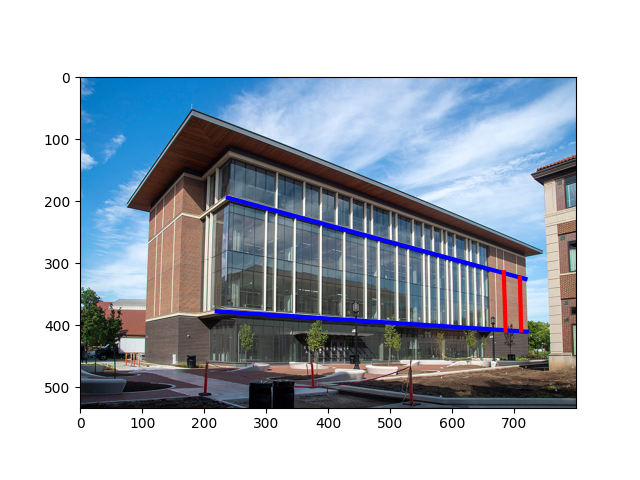
\includegraphics[width=0.45\textwidth]{../building_transformed_2_step_parallel_lines.png}}
    \subcaptionbox{\large\textbf{b}}{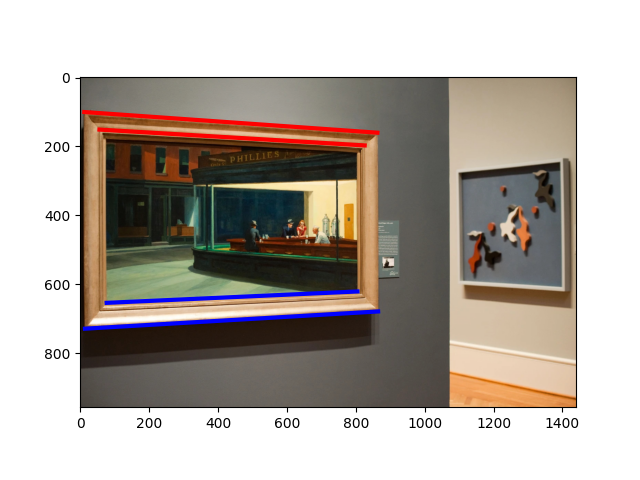
\includegraphics[width=0.45\textwidth]{../nighthawks_transformed_2_step_parallel_lines.png}}
    \caption{Parallel Line Segments (shown in blue and red color)}
    \label{fig:parallel_lines}
\end{figure}
The corresponding homography matrices and images are shown in the next Fig. \ref{fig:2_step_1(1)} and \ref{fig:2_step_1(2)}.
\begin{equation*}
	H_{projective} = \begin{bmatrix}
	1 & 0 & 0\\ 0 & 1 & 0\\-8.47809470e-04 & -9.96459304e-05 &1
	\end{bmatrix}
\end{equation*}
\begin{figure}[!htbp]
     \centering
    \captionsetup[subfigure]{labelformat=empty}
    \subcaptionbox{\large\textbf{a}}{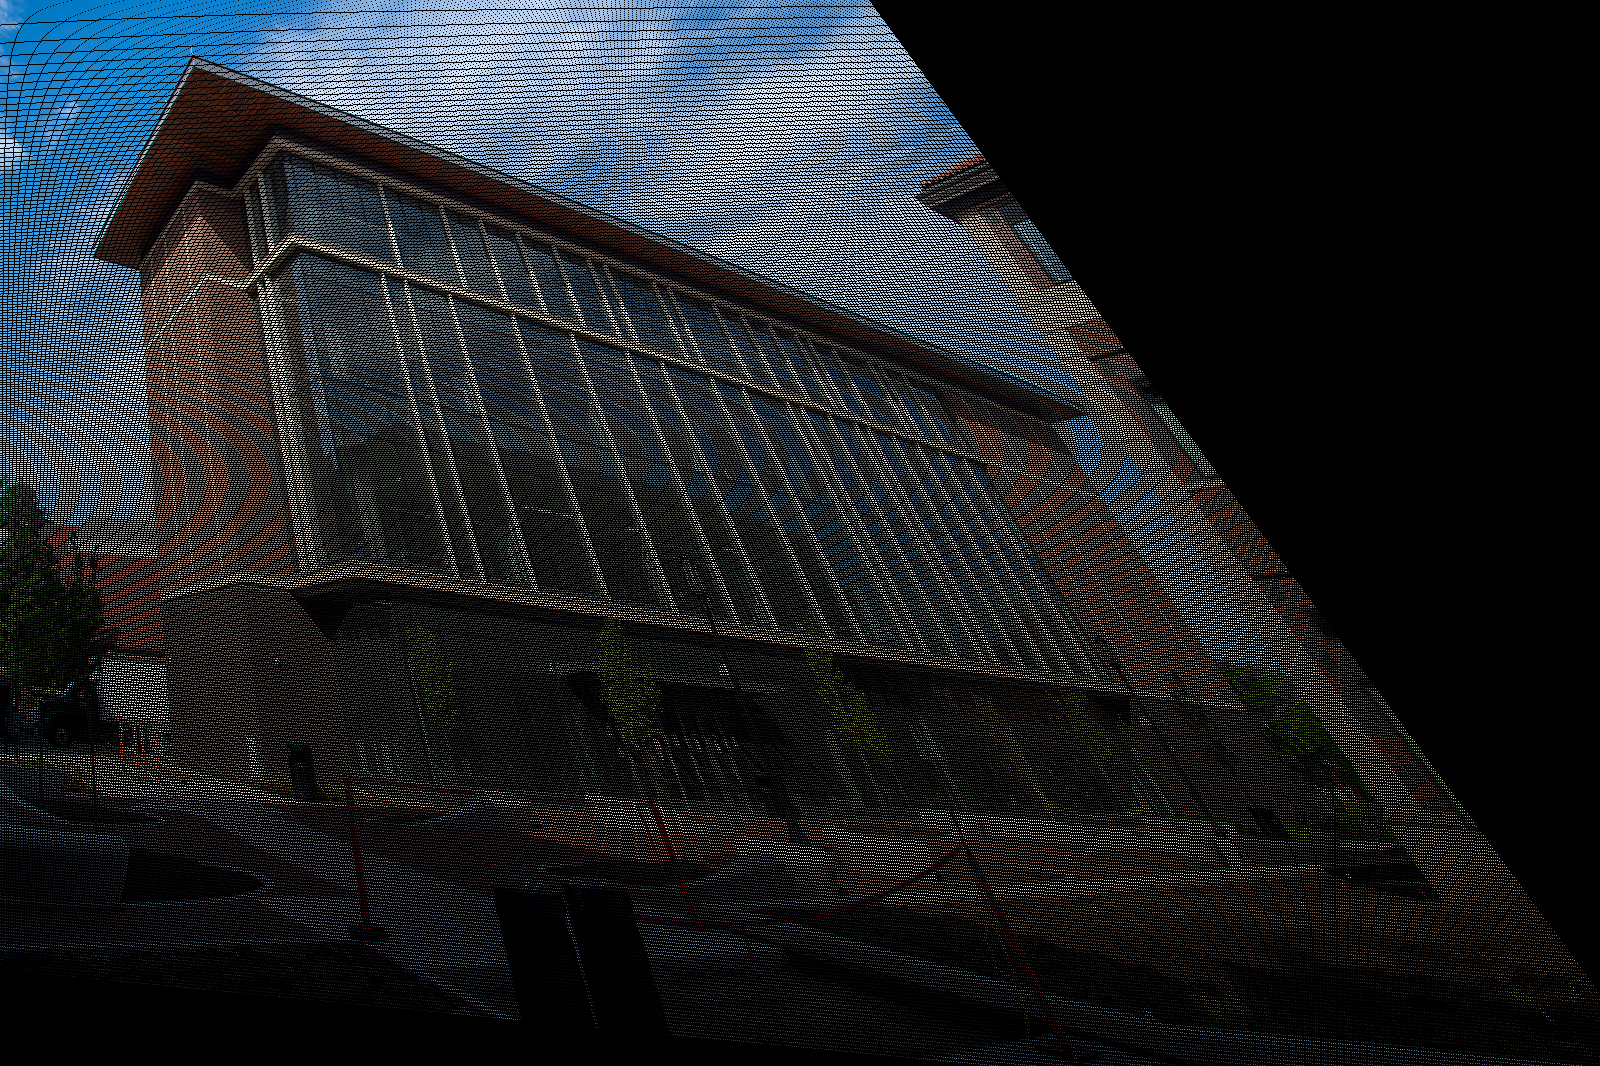
\includegraphics[width=0.45\textwidth]{../building_transformed_2_step_1.png}}
    \caption{Removal of projective distortion in the two step method.}
    \label{fig:2_step_1(1)}
\end{figure}
\newpage
\begin{equation*}
	H_{projective} = \begin{bmatrix}
	1 & 0 & 0\\ 0 & 1 & 0\\-9.25390201e-06 & -2.29916120e-03 & 1
	\end{bmatrix}
\end{equation*}
\begin{figure}[!htbp]
     \centering
    \captionsetup[subfigure]{labelformat=empty}
    \subcaptionbox{\large\textbf{b}}{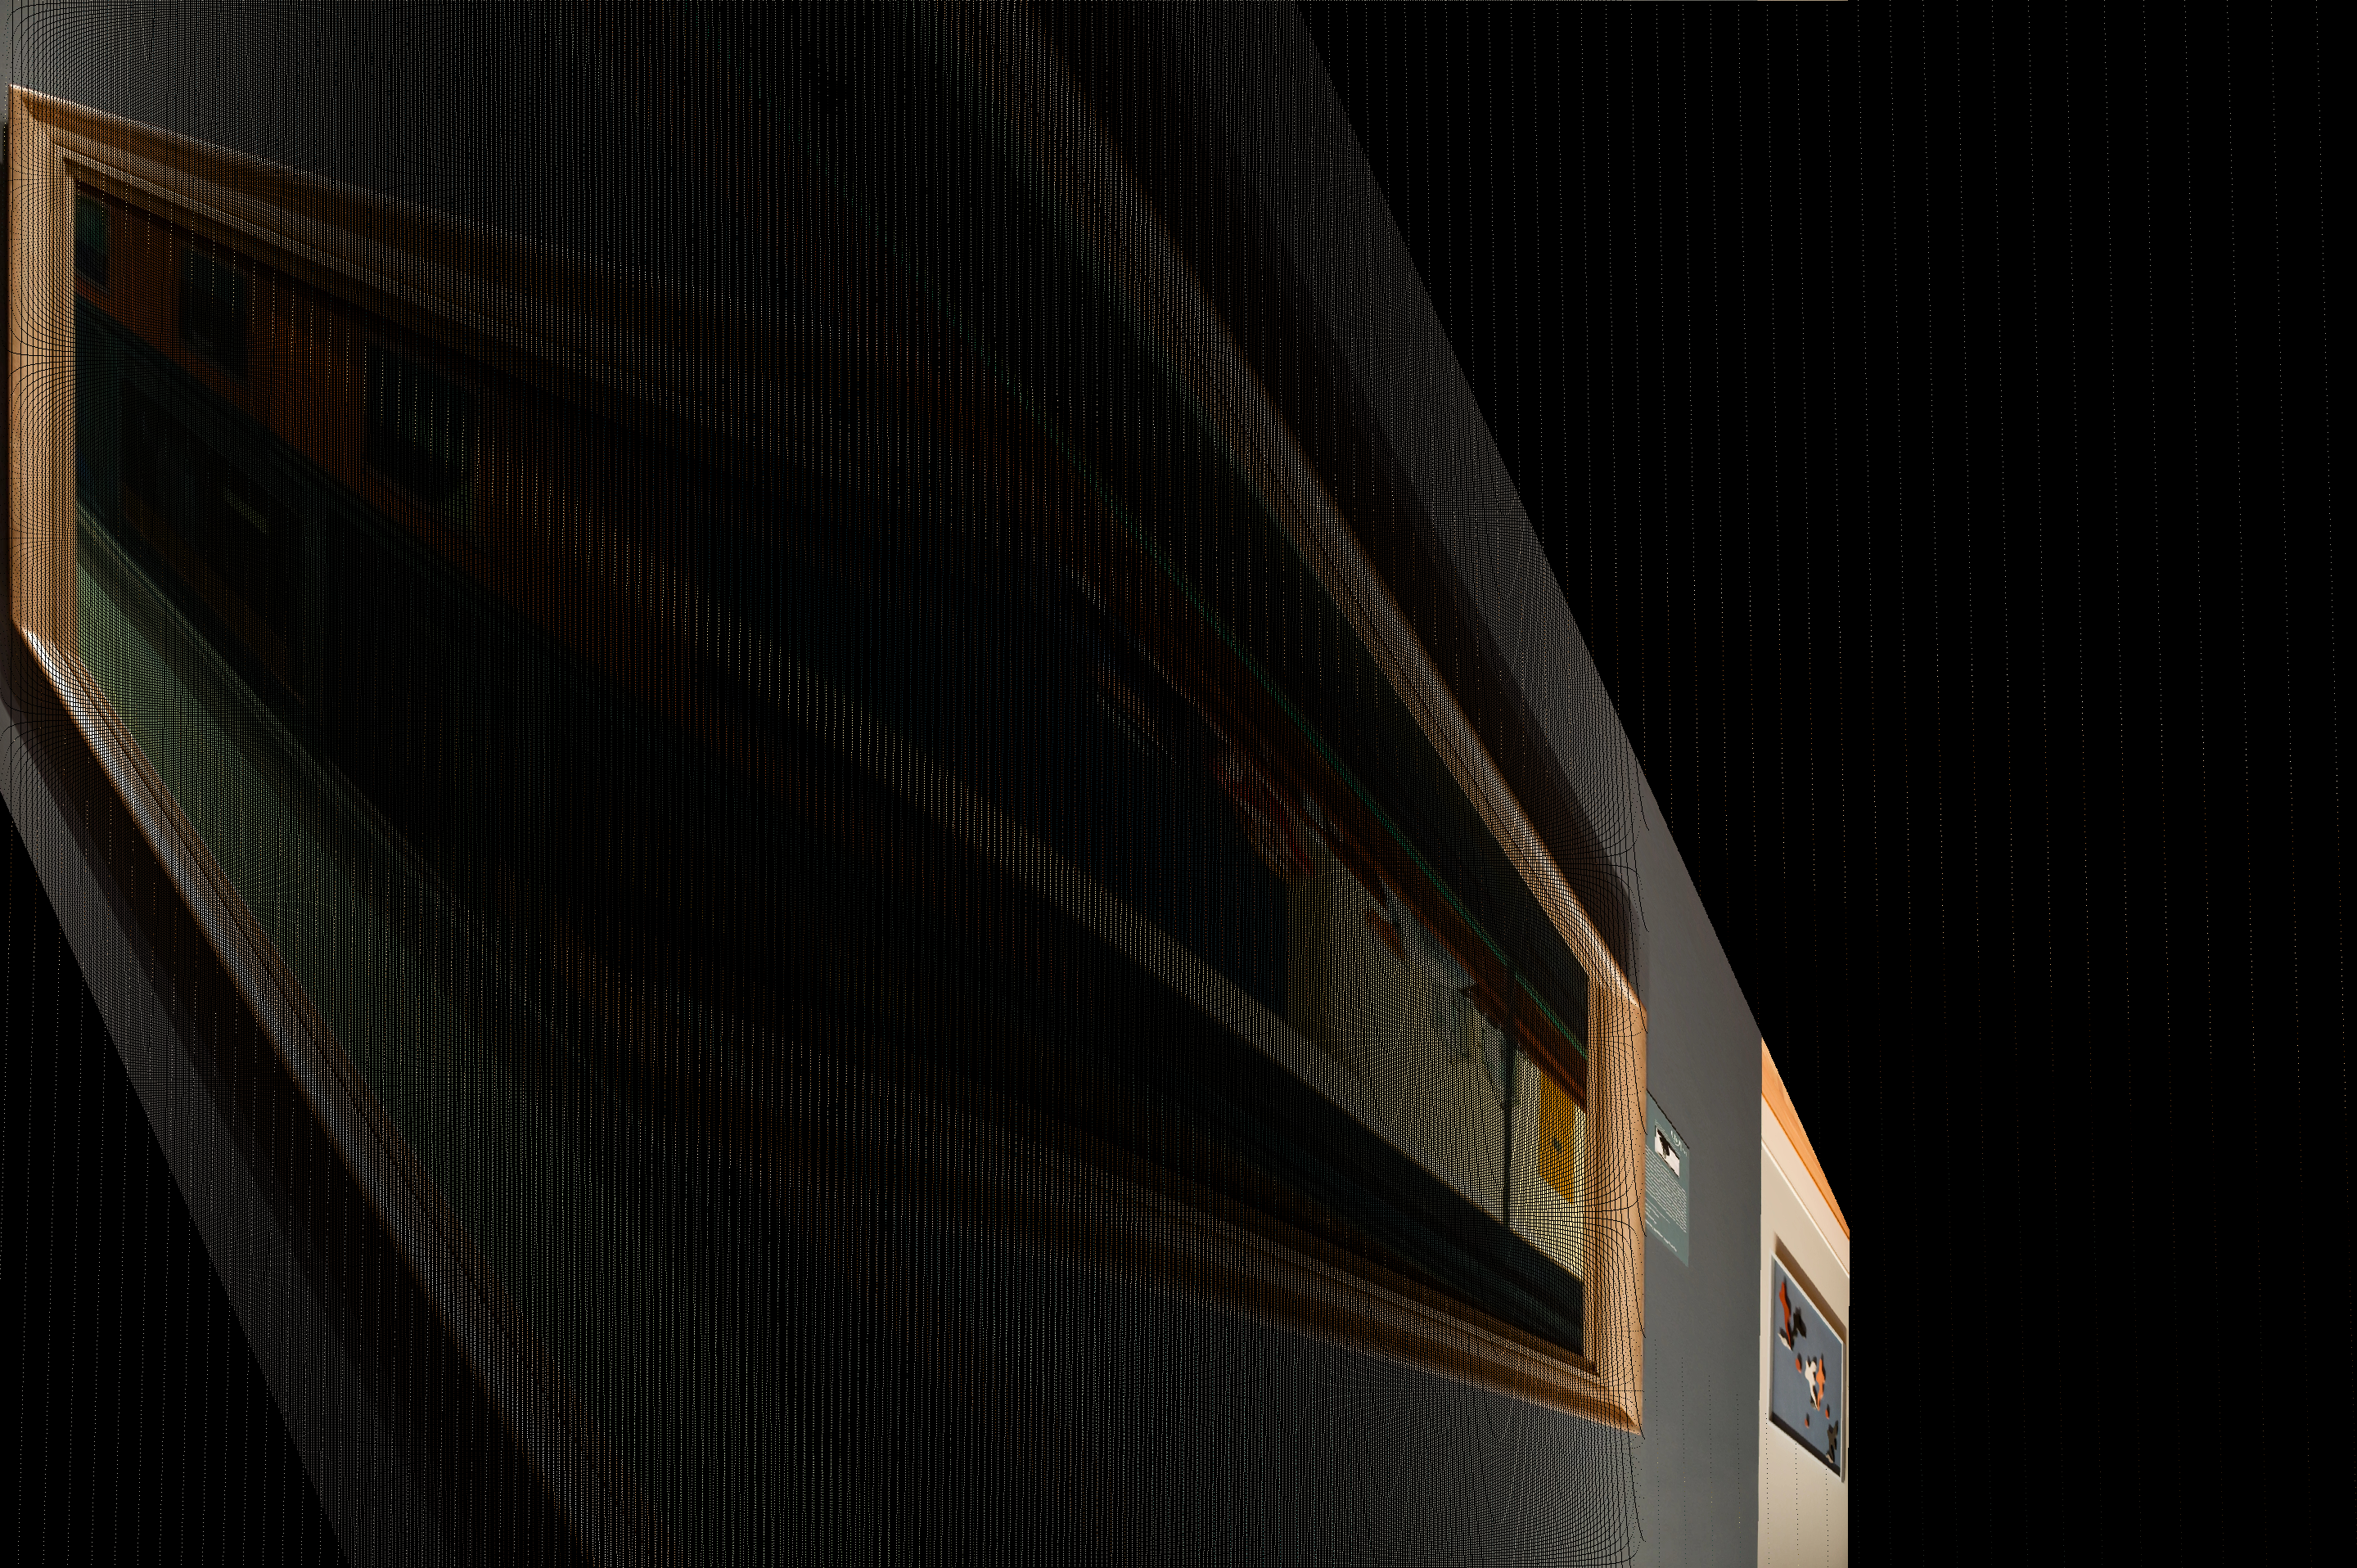
\includegraphics[width=0.45\textwidth]{../nighthawks_transformed_2_step_1.png}}
    \caption{Removal of projective distortion in the two step method.}
    \label{fig:2_step_1(2)}
\end{figure}
\newpage
Two perpendicular lines $l$ and $m$  have the following relationship-
\begin{equation}
cos(\theta) = \frac{l^TC_\infty^*m}{\sqrt{l^TC_\infty^*l m^TC_\infty^*m]}} = 0.
\end{equation}
Using the homographic transformation $l'=H^{-T}l$ and $m'=H^{-T}m$, we can form the following relationship-
\begin{equation}
	l'^THC^*_\infty H^Tm' = 0
\end{equation}
Since, $H$ is an affine transformation, $H$ has the form of
\begin{equation}
	H = \begin{bmatrix}
		A & t \\ 0^T & 1
	\end{bmatrix}
\end{equation}
Plugging in all the terms, we have-
\begin{equation}
	0 = \begin{bmatrix}l_1' & l_2' & l_3'\end{bmatrix} \begin{bmatrix}AA^T & 0 \\ 0^T & 0\end{bmatrix}\begin{bmatrix}m_1' \\ m_2' \\ m_3'\end{bmatrix}
\end{equation}
Considering $S=\begin{bmatrix}AA^T & 0 \\ 0^T & 0\end{bmatrix}=\begin{bmatrix}s_{11} & s_{12} \\ s_{12} & 1\end{bmatrix}$, we have-
\begin{equation}
	s_{11}l_1'm_1' + s_{12}(l_1'm_2' + l_2'm_1') = -l_2'm_2'
\end{equation}
We can find the unknown coefficients of $S$ matrix if we have two pairs of perpendicular lines. Fig. \ref{fig:perpendicular_lines} shows the choice of these perpendicular line segments in red and blue colors.
\begin{figure}[!htbp]
     \centering
    \captionsetup[subfigure]{labelformat=empty}
    \subcaptionbox{\large\textbf{b}}{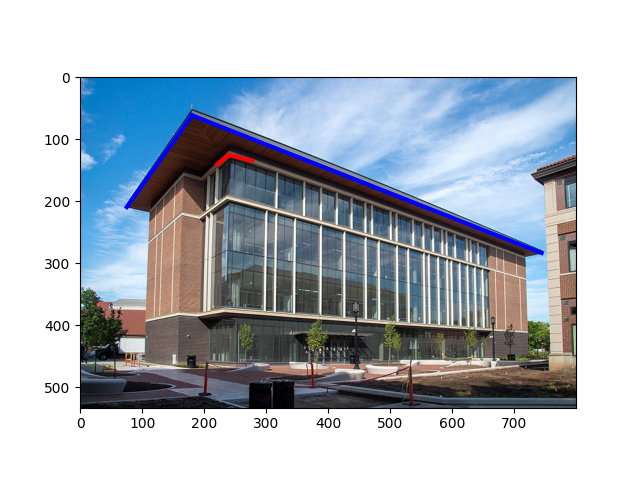
\includegraphics[width=0.45\textwidth]{../building_transformed_2_step_perpendicular_lines.png}}
    \subcaptionbox{\large\textbf{b}}{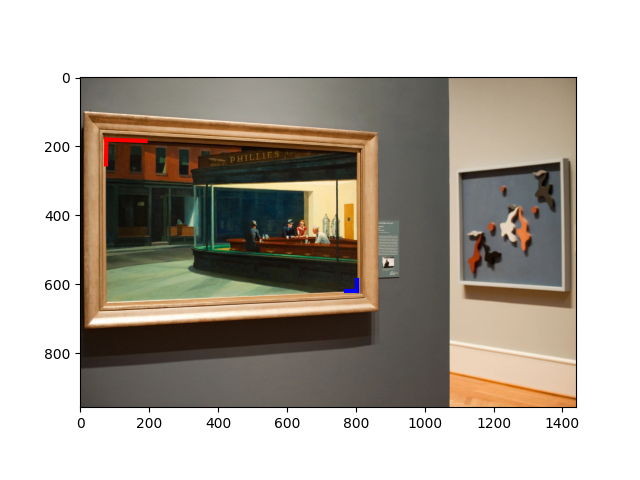
\includegraphics[width=0.45\textwidth]{../nighthawks_transformed_2_step_perpendicular_lines.png}}
    \caption{Choice of perpendicular lines for affine distortion removal.}
    \label{fig:perpendicular_lines}
\end{figure}
The affine distortion removal homography matrices and the final undistorted images are shown in Fig. \ref{fig:2_step_2(1)} and \ref{fig:2_step_2(2)}. Note: The final undistorted images are formed by multiplication of $H_{affine}$ and $H_{distirtive}$ to the initial distorted image.
\begin{equation*}
	H_{affine} = \begin{bmatrix}
	0.91690833 & 0.57676063 & 0\\ 0.57676063 & 0.8169132 & 0\\0 & 0 & 1
	\end{bmatrix}
\end{equation*}
\begin{figure}[!htbp]
     \centering
    \captionsetup[subfigure]{labelformat=empty}
    \subcaptionbox{\large\textbf{a}}{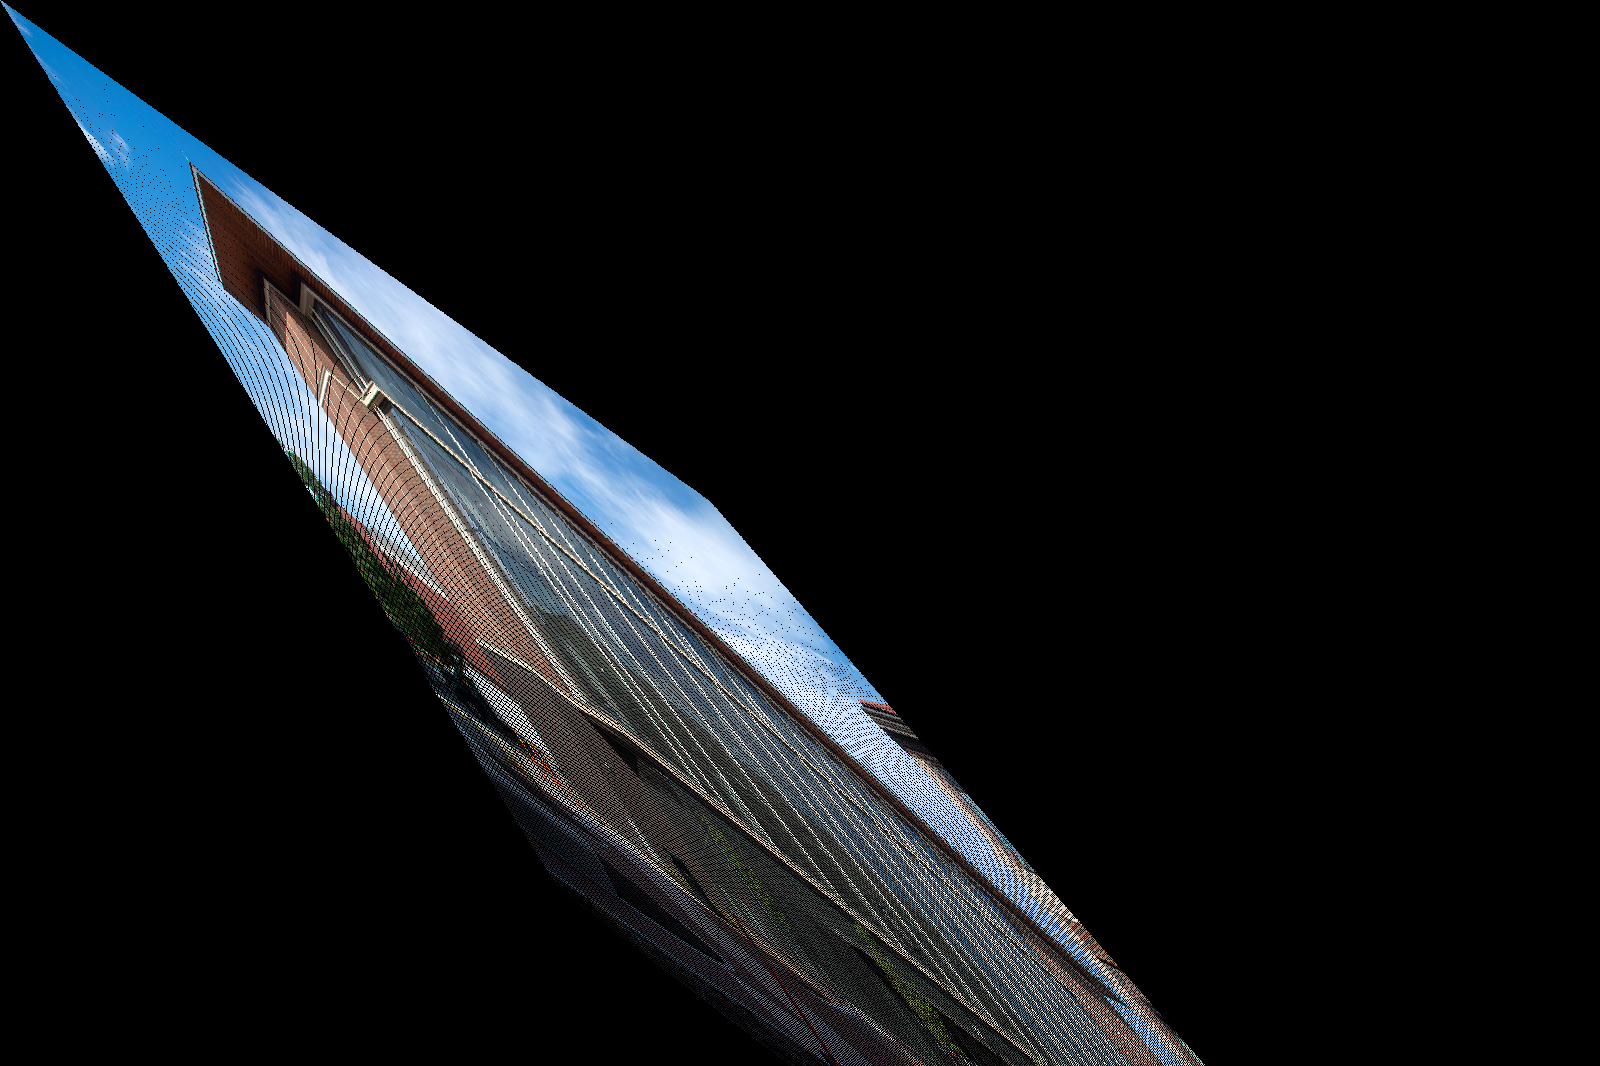
\includegraphics[width=0.45\textwidth]{../building_transformed_2_step_2.png}}
    \caption{Removal of both projective abd affine distortion in the two step method.}
    \label{fig:2_step_2(1)}
\end{figure}
\begin{equation*}
	H_{affine} = \begin{bmatrix}
	1 & 0 & 0\\ 0 & 1 & 0\\0&0 & 1
	\end{bmatrix}
\end{equation*}
\begin{figure}[!htbp]
     \centering
    \captionsetup[subfigure]{labelformat=empty}
    \subcaptionbox{\large\textbf{b}}{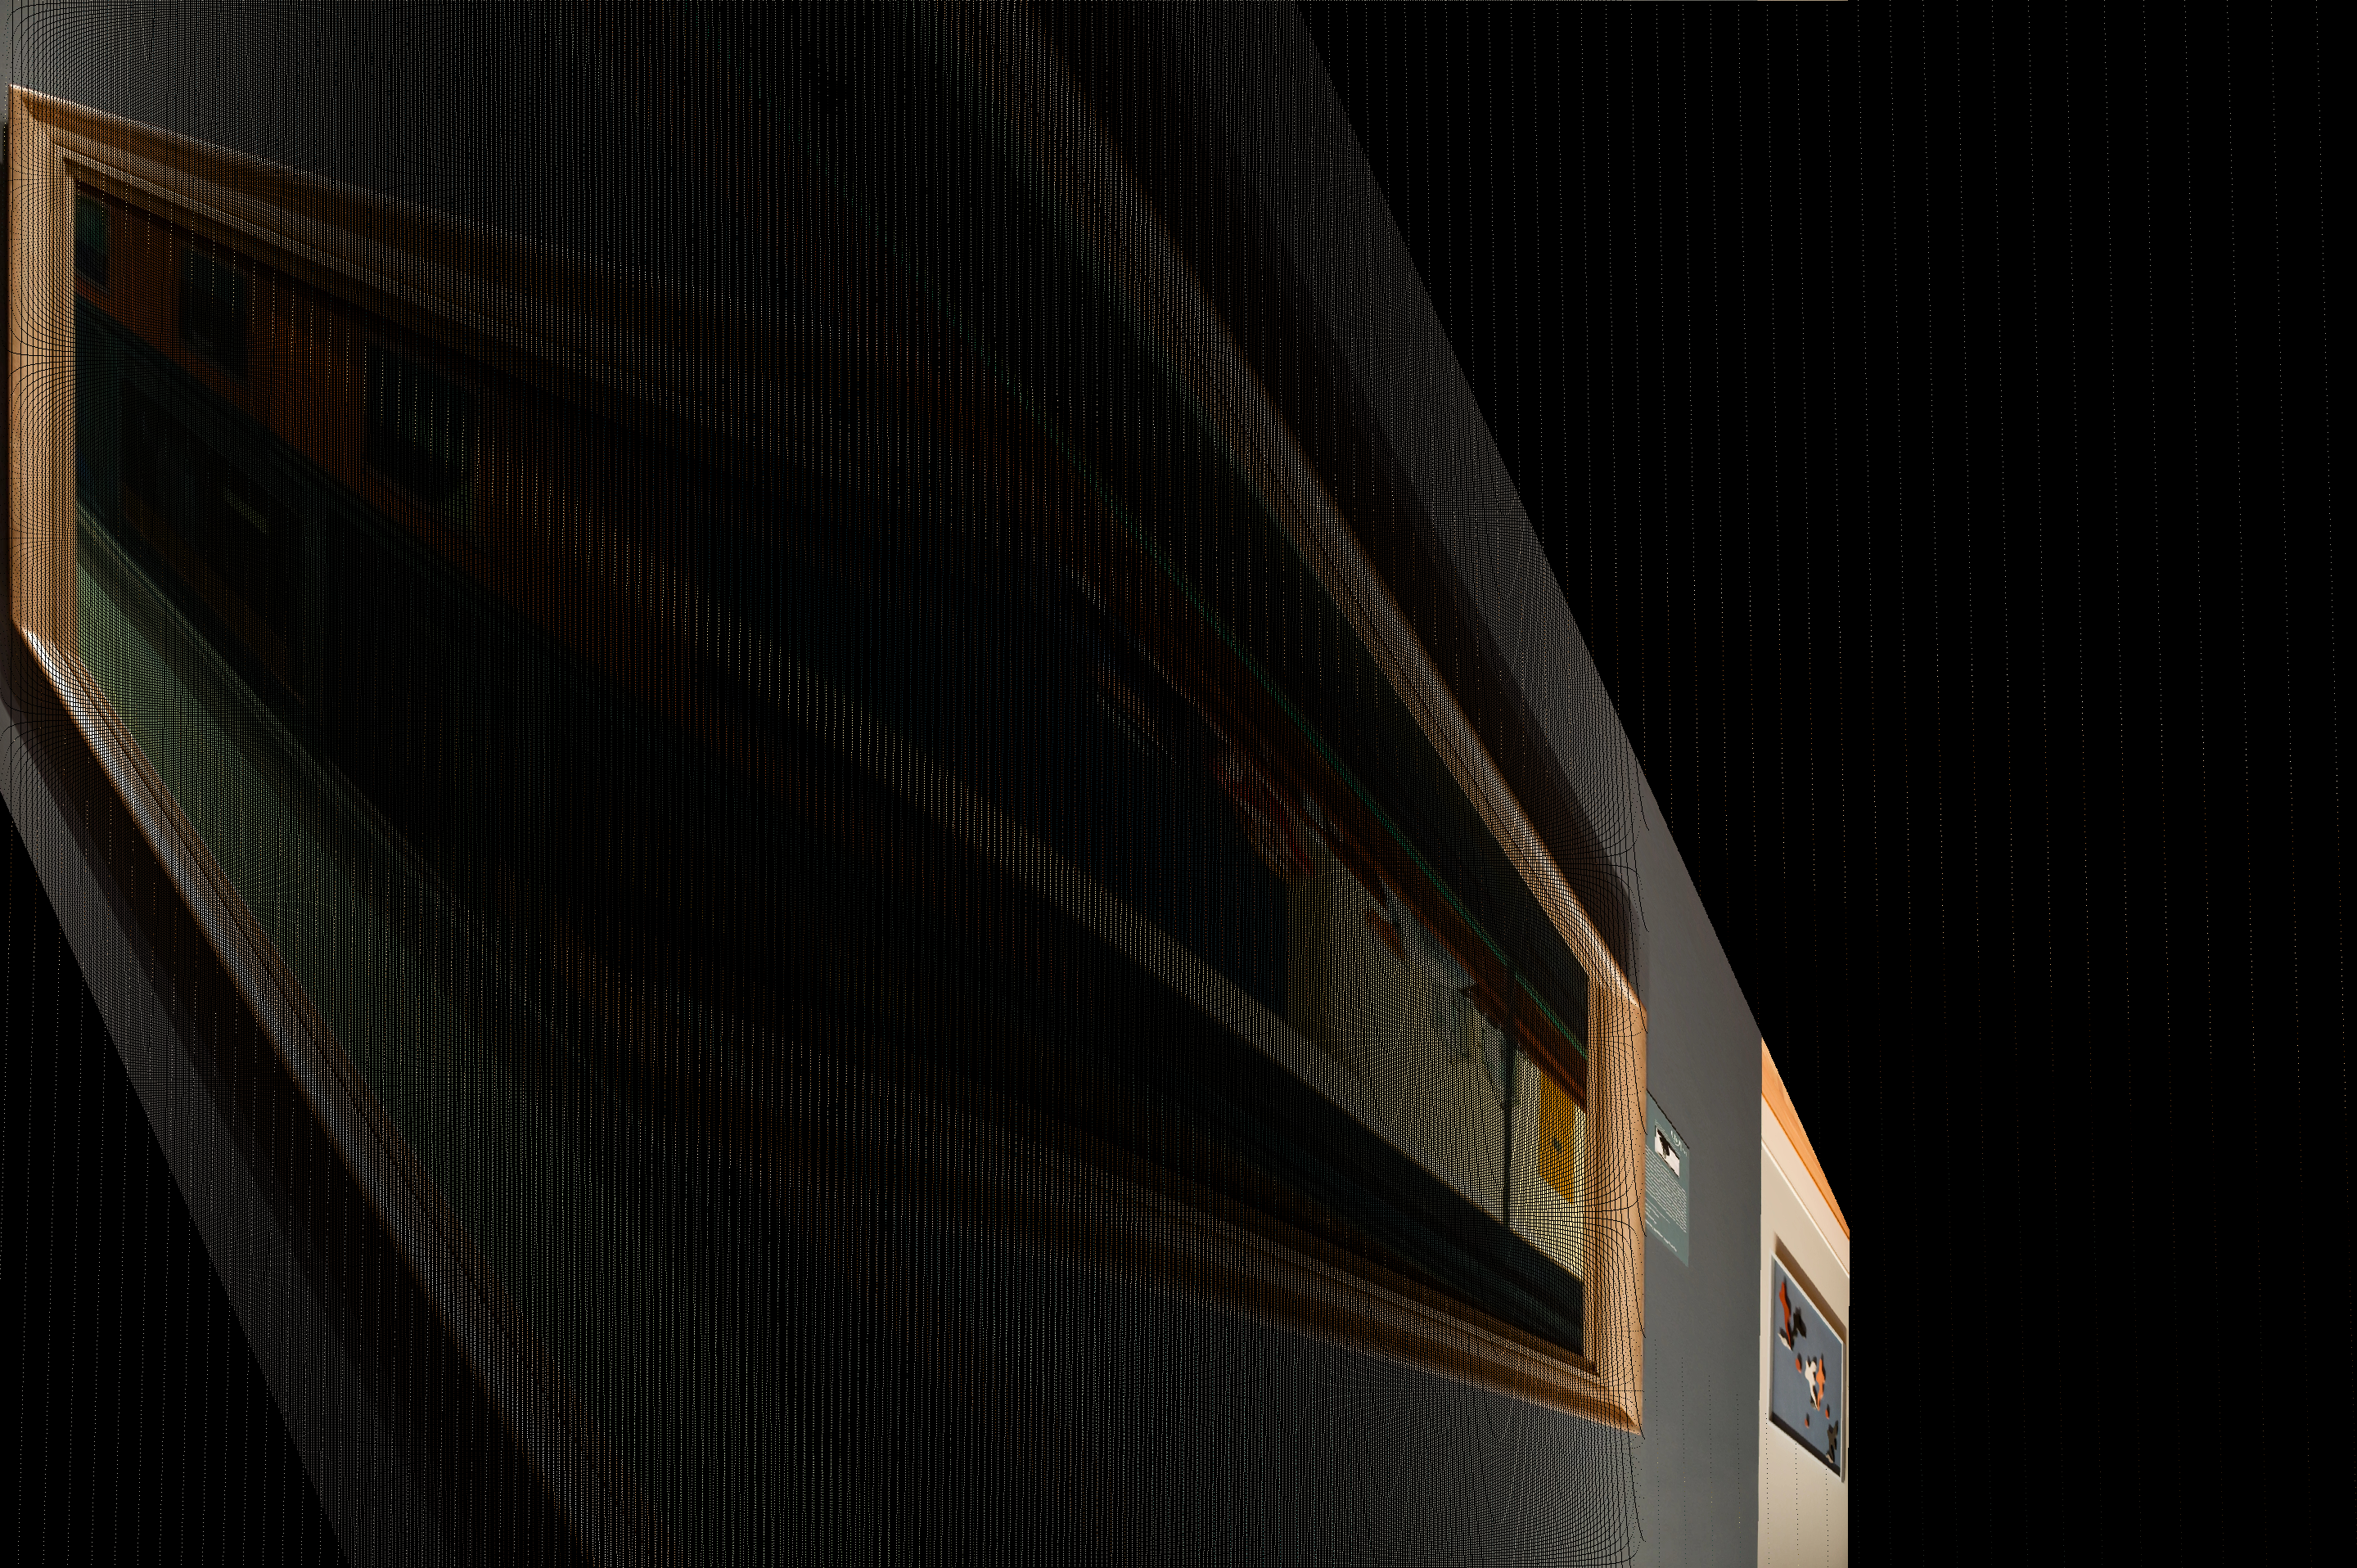
\includegraphics[width=0.45\textwidth]{../nighthawks_transformed_2_step_2.png}}
    \caption{Removal of both projective abd affine distortion in the two step method.}
    \label{fig:2_step_2(2)}
\end{figure}


\newpage
\subsection{Source Code}
\begin{lstlisting}[language=Python]
import numpy as np
import matplotlib.pyplot as plt
import matplotlib.image as mpimg
import matplotlib.patches as patches
from PIL import Image
import scipy.ndimage as ndimage


card1 = mpimg.imread('./card1.jpeg')
card2 = mpimg.imread('./card2.jpeg')
card3 = mpimg.imread('./card3.jpeg')
car = mpimg.imread('./car.jpg')

'''
print(car.shape)
imgplot = plt.imshow(car)
# Create a Rectangle patch
rect = patches.Rectangle((21, 31), 700, 500, linewidth=1, edgecolor='r', facecolor='none')
# Add the patch to the Axes
ax = plt.gca();
ax.add_patch(rect)
plt.savefig('car_bounding_box.png')
#plt.show()
'''

#Physical coordinates
card1_coord = np.array([[488,252],[610,1114],[1220,800],[1241,177]])
card2_coord = np.array([[318,230],[218,864],[872,1128],[1042,232]])
card3_coord = np.array([[586,47],[61,591],[701,1214],[1230,675]])
car_coord = np.array([[21,31],[21,531],[721,531],[721,31]])

def homography_coefficients(input_coord,target_coord,mode=None):
	A = np.array([[input_coord[0,0],input_coord[0,1],1,0,0,0,-input_coord[0,0]*target_coord[0,0],-input_coord[0,1]*target_coord[0,0]],\
	[0,0,0,input_coord[0,0],input_coord[0,1],1,-input_coord[0,0]*target_coord[0,1],-input_coord[0,1]*target_coord[0,1]],\
	[input_coord[1,0],input_coord[1,1],1,0,0,0,-input_coord[1,0]*target_coord[1,0],-input_coord[1,1]*target_coord[1,0]],\
	[0,0,0,input_coord[1,0],input_coord[1,1],1,-input_coord[1,0]*target_coord[1,1],-input_coord[1,1]*target_coord[1,1]],\
	[input_coord[2,0],input_coord[2,1],1,0,0,0,-input_coord[2,0]*target_coord[2,0],-input_coord[2,1]*target_coord[2,0]],\
	[0,0,0,input_coord[2,0],input_coord[2,1],1,-input_coord[2,0]*target_coord[2,1],-input_coord[2,1]*target_coord[2,1]],\
	[input_coord[3,0],input_coord[3,1],1,0,0,0,-input_coord[3,0]*target_coord[3,0],-input_coord[3,1]*target_coord[3,0]],\
	[0,0,0,input_coord[3,0],input_coord[3,1],1,-input_coord[3,0]*target_coord[3,1],-input_coord[3,1]*target_coord[3,1]]])

	b = np.array([[target_coord[0,0]],[target_coord[0,1]],[target_coord[1,0]],[target_coord[1,1]],[target_coord[2,0]],[target_coord[2,1]],[target_coord[3,0]],[target_coord[3,1]]])
	x = np.matmul(np.linalg.inv(A),b)

	H = np.zeros((3,3))
	H[0,0] = x[0]
	H[0,1] = x[1]
	H[0,2] = x[2]
	H[1,0] = x[3]
	H[1,1] = x[4]
	H[1,2] = x[5]
	H[2,0] = x[6]
	H[2,1] = x[7]
	H[2,2] = 1
	if mode=='affine':
		H[2,0] = 0
		H[2,1] = 0
	return H

def transform_image(H,input_image,target_image):
	transformed_image = np.ones(target_image.shape)*255
	for i in range(0,input_image.shape[0]):
		for j in range(0,input_image.shape[1]):
			h_coordinate = np.array([j,i,1])
			t = np.matmul(H,h_coordinate)
			t = np.rint(t/t[2])
			t = t.astype('int')
			if (t[0]<target_image.shape[0] and t[1]<target_image.shape[1]):
				transformed_image[t[1],t[0],0] = input_image[i,j,0]
				transformed_image[t[1],t[0],1] = input_image[i,j,1]
				transformed_image[t[1],t[0],2] = input_image[i,j,2]
	'''
	for i in range(1,input_image.shape[0]-1):
		for j in range(1,input_image.shape[1]-1):
			sum0 = 0
			sum1=0
			sum2=0
			for k in range(i-1,i+2):
				for l in range(j-1,j+2):
					sum0 = sum0 + transformed_image[k,l,0]
					sum1 = sum1 + transformed_image[k,l,1]
					sum2 = sum2 + transformed_image[k,l,2]

			transformed_image[i,j,0] = sum0/9
			transformed_image[i,j,1] = sum1/9
			transformed_image[i,j,2] = sum2/9
	'''
	return transformed_image

#########################   Task 1 #############################################
H = homography_coefficients(car_coord,card1_coord)
transformed_image = transform_image(H,car,card1)
transformed_image = transformed_image.astype(np.uint8)
plt.imsave("car_transformed_to_card1.png",transformed_image)

H = homography_coefficients(car_coord,card2_coord)
transformed_image = transform_image(H,car,card2)
transformed_image = transformed_image.astype(np.uint8)
plt.imsave("car_transformed_to_card2.png",transformed_image)

H = homography_coefficients(car_coord,card3_coord)
transformed_image = transform_image(H,car,card3)
transformed_image = transformed_image.astype(np.uint8)
plt.imsave("car_transformed_to_card3.png",transformed_image)

H12 = homography_coefficients(card1_coord,card2_coord)
H23 = homography_coefficients(card2_coord,card3_coord)
transformed_image = transform_image(np.matmul(H23,H12),card1,card3)
transformed_image = transformed_image.astype(np.uint8)
plt.imsave("card1_transformed_to_card3.png",transformed_image)

H = homography_coefficients(car_coord,card1_coord,mode='affine')
transformed_image = transform_image(H,car,card1)
transformed_image = transformed_image.astype(np.uint8)
plt.imsave("car_transformed_to_card1_affine.png",transformed_image)

H = homography_coefficients(car_coord,card2_coord,mode='affine')
transformed_image = transform_image(H,car,card2)
transformed_image = transformed_image.astype(np.uint8)
plt.imsave("car_transformed_to_card2_affine.png",transformed_image)

H = homography_coefficients(car_coord,card3_coord,mode='affine')
transformed_image = transform_image(H,car,card3)
transformed_image = transformed_image.astype(np.uint8)
plt.imsave("car_transformed_to_card3_affine.png",transformed_image)

#########################   Task 2 #############################################
custom_image_1 = mpimg.imread('./custom_image_1.jpg')
custom_image_2 = mpimg.imread('./custom_image_2.jpg')
custom_image_3 = mpimg.imread('./custom_image_3.jpg')
custom_projecting_image = mpimg.imread('./custom_projecting_image.jpg')
#Physical coordinates
custom_image_1_coord = np.array([[658,353],[31,1230],[2932,1352],[2717,320]])
custom_image_2_coord = np.array([[831,332],[49,1216],[2618,1726],[2873,445]])
custom_image_3_coord = np.array([[278,660],[341,2146],[2704,2476],[2719,250]])
custom_projecting_image_coord = np.array([[235,424],[140,2025],[2736,2186],[2722,409]])
#plt.imshow(custom_projecting_image)
#plt.show()

H = homography_coefficients(custom_projecting_image_coord,custom_image_1_coord)
transformed_image = transform_image(H,custom_projecting_image,custom_image_1)
transformed_image = transformed_image.astype(np.uint8)
plt.imsave("cst_transformed_to_cst1.png",transformed_image)

H = homography_coefficients(custom_projecting_image_coord,custom_image_2_coord)
transformed_image = transform_image(H,custom_projecting_image,custom_image_2)
transformed_image = transformed_image.astype(np.uint8)
plt.imsave("cst_transformed_to_cst2.png",transformed_image)

H = homography_coefficients(custom_projecting_image_coord,custom_image_3_coord)
transformed_image = transform_image(H,custom_projecting_image,custom_image_3)
transformed_image = transformed_image.astype(np.uint8)
plt.imsave("cst_transformed_to_cst3.png",transformed_image)

H12 = homography_coefficients(custom_image_1_coord,custom_image_2_coord)
H23 = homography_coefficients(custom_image_2_coord,custom_image_3_coord)
transformed_image = transform_image(np.matmul(H23,H12),custom_image_1,custom_image_3)
transformed_image = transformed_image.astype(np.uint8)
plt.imsave("cst1_transformed_to_cst3.png",transformed_image)

H = homography_coefficients(custom_projecting_image_coord,custom_image_1_coord,mode='affine')
transformed_image = transform_image(H,custom_projecting_image,custom_image_1)
transformed_image = transformed_image.astype(np.uint8)
plt.imsave("cst_transformed_to_cst1_affine.png",transformed_image)

H = homography_coefficients(custom_projecting_image_coord,custom_image_2_coord,mode='affine')
transformed_image = transform_image(H,custom_projecting_image,custom_image_2)
transformed_image = transformed_image.astype(np.uint8)
plt.imsave("cst_transformed_to_cst2_affine.png",transformed_image)

H = homography_coefficients(custom_projecting_image_coord,custom_image_3_coord,mode='affine')
transformed_image = transform_image(H,custom_projecting_image,custom_image_3)
transformed_image = transformed_image.astype(np.uint8)
plt.imsave("cst_transformed_to_cst3_affine.png",transformed_image)

\end{lstlisting}
\end{document}
